\documentclass{sig-alternate-05-2015}
\usepackage{amsmath}
\usepackage[]{mcode}
\usepackage[]{algorithm2e}
\usepackage[T1]{fontenc}
\newcommand\numberthis{\addtocounter{equation}{1}\tag{\theequation}}
\lstset{numbers = left}

\begin{document}

\author{Alun Meredith\vspace{-2ex}% Toggle commenting out the command
}
\title{Options Pricing \vspace{-2ex}% to see the effect
}
\maketitle

\vspace{-30mm}
\small
\begin{abstract}
In this paper we replicate an Radial Basis Function model build by Hutchinson \textit{et. al} \cite{hutchinson1994nonparametric} and replicate their results. We find that this model can accurately replicate call option values, Black-Scholes call option values and associated deltas with R squared values greater than 0.90. 
\end{abstract}
\normalsize
\section{Introduction}
Hutchinson \textit{et. al} \cite{hutchinson1994nonparametric} proposes that the relationship between option price and its parameters can be approximated through non-parametric approaches. They use Monte Carlo simulations to train a variety of models to approximate the Black-Scholes closed form solution and explore the performance of predicting observed call prices on a Historic data. They compare the different models through their out of sample R squared values and find that a Radial Basis function model has the best performance. 

In this paper we replicate parts of their paper, training an RBF model on historic option prices of the FTSE index and compare the resultant out of sample R squared values to those found by Hutchinson \textit{et. al} and calculate deltas implied from this model. We also train the model on the Black-Scholes call values and deltas and evaluate its ability to approximate these. 

%\subsection*{Use Gaussian Mixture Modelling to create non-linear mapping}

To create a non-linear transformation of the data Gaussian Mixture Modelling (GMM) was conducted using an Expectation-Maximisation algorithm, under the restrictions of 4 centres with equal covariance matrices. Figure \ref{fig:RBF} shows how the distribution is characterised by these centres. Hutchinson \textit{et. al} \cite{hutchinson1994nonparametric} uses this restriction of centres to minimise over-fitting.  

\begin{figure}[h]
	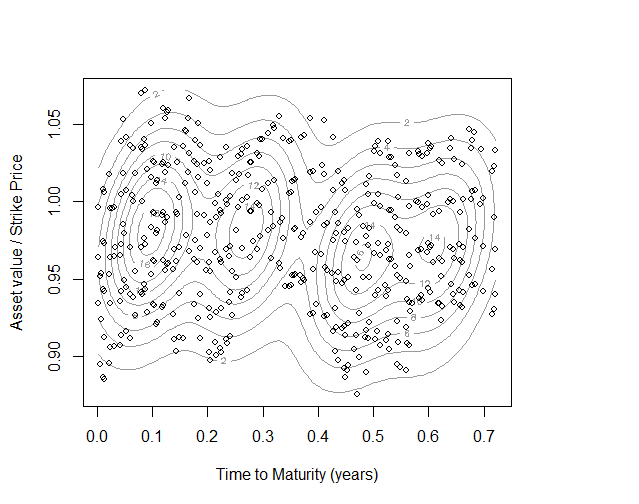
\includegraphics[width=\linewidth]{RBF.png}
	\centering
	\caption{Probability distribution described by Gaussian Mixture Model}
			\label{fig:RBF}
\end{figure} 

Extracting the centres and covariance from the GMM, non-linear features of the observations were built as the Mahalanobis distance to each center. A linear model of these features in addition to the linear features can be defined as:

\begin{align}
c = \sum^J_{j=1}\lambda_j\phi_j(\mathbf{x}) + \mathbf{\omega^Tx} + \omega_0 \label{eq:1}
\end{align}

Where $\mathbf{x} = [(T-t)\ \ S/X]^T$\footnote{Note: During coding I realised I inverted the order of the linear features and was easier to keep it this way} and $\phi_j(\mathbf{x})$ is the non-linear mapping describing the Mahalanobis distance (without a bias term) to each of the trained centres:

\begin{align}
\phi_j(\mathbf{x}) = \left[(\mathbf{x - m_j})^T \mathbf{\Sigma} (\mathbf{s - m_j})\right]^{1/2} 
\end{align}

To find the weights of this linear model a design matrix was constructed and the squared error minimised by solving the least squared problem below:

\begin{align}
\begin{bmatrix}
  \phi_1 & \phi_2 & \phi_3 & \phi_4 & S/X & T-t & 1 \\ 
  \vdots & \vdots & \vdots & \vdots & \vdots & \vdots & \vdots \\ 
  \vdots & \vdots & \vdots & \vdots & \vdots & \vdots & \vdots \\ 
\end{bmatrix}
\begin{bmatrix}
  \lambda_1 \\ 
  \lambda_2 \\ 
  \lambda_3 \\ 
  \lambda_1 \\ 
  w_1 \\ 
  w_2 \\ 
  w_0 \\ 
  \end{bmatrix} = \mathbf{c}
\end{align}

In \eqref{eq:1} the Black-Scholes call price was trained but we also evaluate the model trained against the historic call values and Black-Scholes deltas (derivative of call price w.r.t. asset value). The implicit value of delta $\left(\Delta = \frac{\partial c}{\partial S}\right)$ in the model can be found by finding the derivative of \eqref{eq:1}:

\begin{align*}
\frac{\partial c}{\partial S} = \sum^J_{j=1} \lambda_j \frac{\partial \phi_j}{\partial S} + \mathbf{w}^T \frac{\partial \mathbf{x}}{\partial S} \\
\frac{\partial x}{\partial S} = [0 \ 1/X]^T \\
\phi = \sqrt{\mathbf{(x-\mu)}^T\mathbf{\Sigma(x-\mu)}} = \sqrt{\mathbf{f}} \\
\frac{\partial \phi}{\partial S} = \frac{\partial f}{\partial S} \frac{\partial \phi}{\partial f} \\
\frac{\partial \phi}{\partial f} = \frac{1}{2} f^{-1/2} \\
f = \mathbf{a^T\Sigma a} \qquad where \qquad \mathbf{a = (x - \mu)} \\
\frac{\partial f}{\partial S} = \frac{\partial f}{\partial a} \frac{\partial a}{\partial S} \\
\frac{\partial f}{\partial S} = \frac{\partial x}{\partial S} =
\frac{\partial f}{\partial S} = 2a^T\Sigma \frac{\partial x}{\partial S} \\
\frac{\partial \phi}{\partial S} = \frac{1}{2}\left[\left(\mathbf{(x-\mu)}^T\mathbf{\Sigma(x-\mu)}\right)^{-1/2} \times 2\mathbf{(x-\mu)}^T\frac{\partial x}{\partial S}\right] \\
\frac{\partial c}{\partial S} = \sum^J_{j=1}\lambda_j \frac{\mathbf{(x-\mu)}^T\frac{\partial x}{\partial S}}{\sqrt{\mathbf{(x-\mu)}^T\mathbf{\Sigma(x-\mu)}}}  + \mathbf{\omega}^T\frac{\partial x}{\partial S} \\
\label{eq:2}
\end{align*}
 
\section{Results}

We trained and evaluated the model using 5 FTSE-100 index call options, with different strike prices, simultaneously running from February to November 1992. The first T/4 observations are used to estimate historic volatility (with a sliding window) to evaluate the Black-Scholes closed form solution. Of the remaining 0.75T observations 60\% are randomly sampled as training data with the remaining 40\% used to test out of sample performance.   

\begin{table}[ht]
\centering
\begin{tabular}{rrr}
  \hline
 & train & test \\ 
  \hline
Vs. BS & 0.92 & 0.91 \\ 
  $\Delta$ (derived) & 0.78 & 0.78 \\ 
  $\Delta$ (trained) & 0.91 & 0.89 \\ 
  Vs. Hist & 0.93 & 0.92 \\ 
  BS v. Hist &  & 0.83 \\ 
   \hline
\end{tabular}
\caption{$R^2$ values of model trained against: BS prices, BS deltas, Historic prices and BS against Historic prices}
\end{table}


\begin{table}[ht]
\centering
\begin{tabular}{rrrr}
  \hline
 & BS & Delta & Hist \\ 
  \hline
$w_0$ & -0.43552 & -4.89332 & -0.44531 \\ 
  $\lambda_1$ & 0.00502 & 0.01434 & 0.00647 \\ 
  $\lambda_2$ & 0.00960 & 0.06798 & 0.00305 \\ 
  $\lambda_3$ & 0.00004 & 0.00351 & -0.00219 \\ 
  $\lambda_4$ & -0.00469 & -0.03814 & -0.00049 \\ 
  $w_2$ & 0.06684 & 0.63737 & 0.01026 \\ 
  $w_1$ & 0.39266 & 4.90705 & 0.44798 \\ 
   \hline
\end{tabular}
\caption{weights of each model}
\end{table}

\begin{table}[ht]
\centering
\begin{tabular}{rrr}
  \hline
 & t\_mat & S/X \\ 
  \hline
  $m_1$ & 0.634 & 0.980 \\ 
  $m_2$ & 0.092 & 0.978 \\ 
  $m_3$ & 0.480 & 0.959 \\ 
  $m_4$ & 0.274 & 0.982 \\ 
   \hline
\end{tabular}
\caption{Position of RBF centres}
\end{table}

\begin{table}[ht]
\centering
\begin{tabular}{rrr}
  \hline
 & $T-t (10^{-3})$ & $S/X (10^{-3})$ \\ 
  \hline
 $T-t$ & 3.76 & 0.65 \\ 
  $S/X$ & 0.65 & 1.79 \\ 
   \hline
\end{tabular}
\caption{Covariance Matrix of RBF centres}
\end{table}


The training set and test set $R^2$ are roughly similar in each model. This suggests that the data is not very overfitted. The choice to use four basis functions was motivated by the desire to minimise over-fitting and this suggests that it was appropriate. 

The $R^2$ values achieved do not meet the ~.99 values of Hutchinson \textit{et. al} using Monte Carlo simulations but when tested on historic data as this report has done they report a value of 93.40 which is roughly equivalent to the findings of this report. Remaining differences are likely due to the larger dataset used. The results reported in this paper shows a BS estimate error with significantly more noise than Hutchinson \textit{et. al} (fig \ref{fig:BS_err}) although they share a similar shape with a peak at S/X = 1 and maturity and a central peak which is approximately a linear function of $t_ma$t and S/X. The noise is likely a result of the underlying data which Hutchinson \textit{et. al} use Monte-Carlo simulations to produce (their figures 4 and 5). 

The $R^2$ produced by training the model on historic data is significantly greater than that of the BS model trained on this data. Confirming the core principal that learnt non-parametric models can often predict relationships better than parametric models at the cost of interpretability.  

The implicit estimation of deltas achieves a reasonable $R^2$ value considering it isn't being directly trained. However looking at the surface there is a systematic effect where high S/X underestimates while low S/X overestimates there are therefore aspects in which the model \eqref{eq:1} doesn't capture the underlying Black-Scholes deltas. 


\section{Conclusion}
We have replicated some of the work of Hutchinson \textit{et. al} \cite{hutchinson1994nonparametric}. We report very similar out of sample R squared values to Hutchinson \textit{et. al} when trained on Historic index data. They achieve 93.26 to our 92.40. This confirms that using historic data that an RBF based learning model can be used to closely approximate both the call option prices and their deltas from the Black-Scholes model. When trained on historic call option values this model achieves higher R squared values than the Black-Scholes model. 

Non-parametric models can better approximate option prices than models such as Black-Scholes but this accuracy is gained at the expense of interpretation. Although some systematic errors in the predictions suggests that the current model isn't able to fully capture the underlying underlying relationship using time to maturity and normalised Asset price. Additional inputs or changes to the features of the model could improve this further. 



\newpage

\begin{figure}[p]
	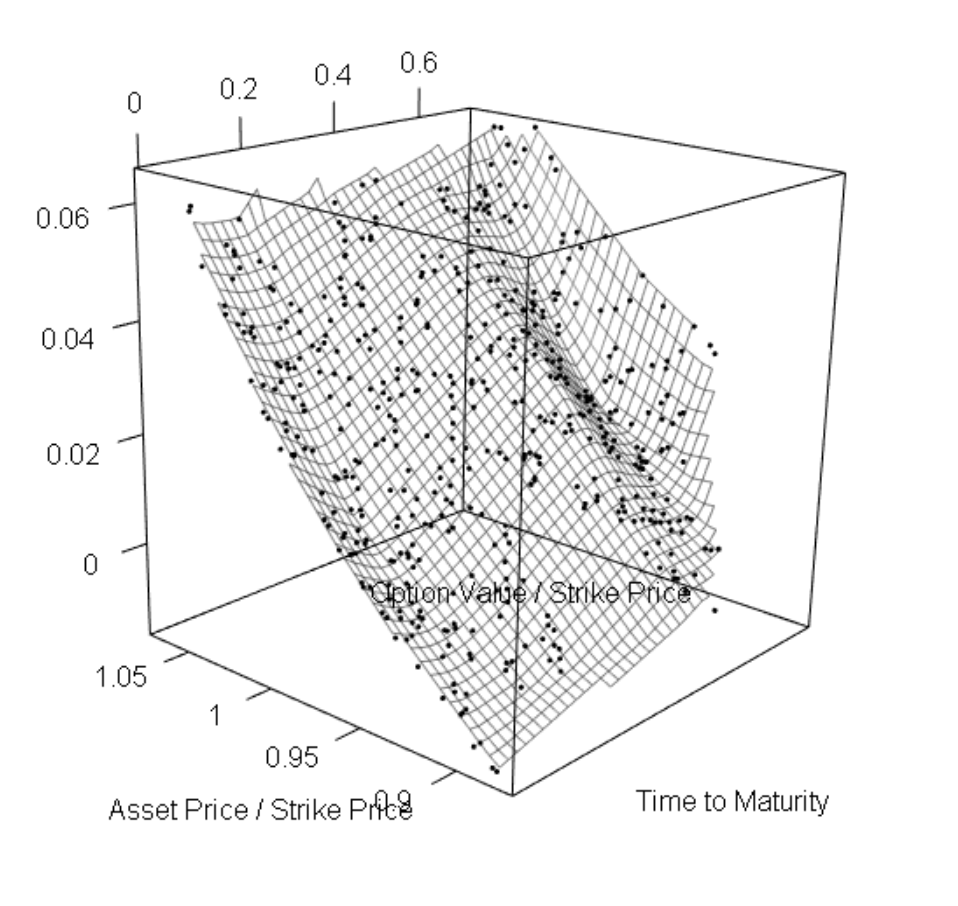
\includegraphics[width=0.7\linewidth]{BS_est.png}
	\centering
	\caption{Model estimation of BS call price}
			\label{fig:BS_est}
\end{figure} 


\begin{figure}[p]
	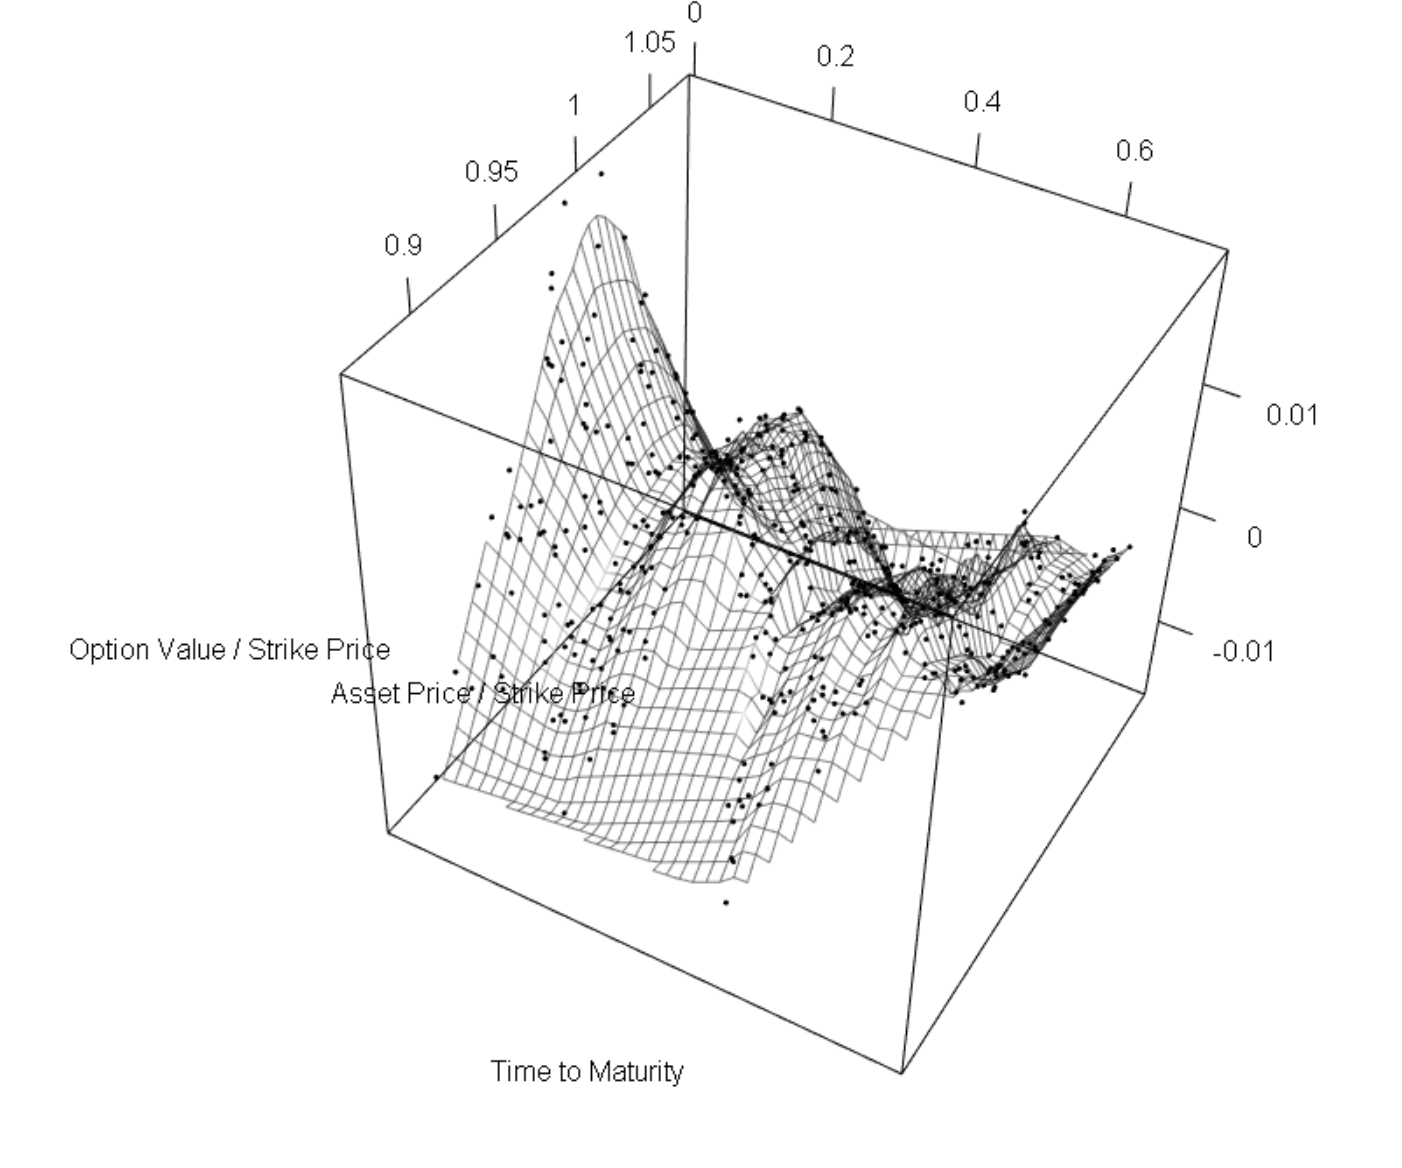
\includegraphics[width=0.7\linewidth]{BS_err.png}
	\centering
	\caption{Model error of BS call price}
			\label{fig:BS_err}
\end{figure} 

\begin{figure}[p]
	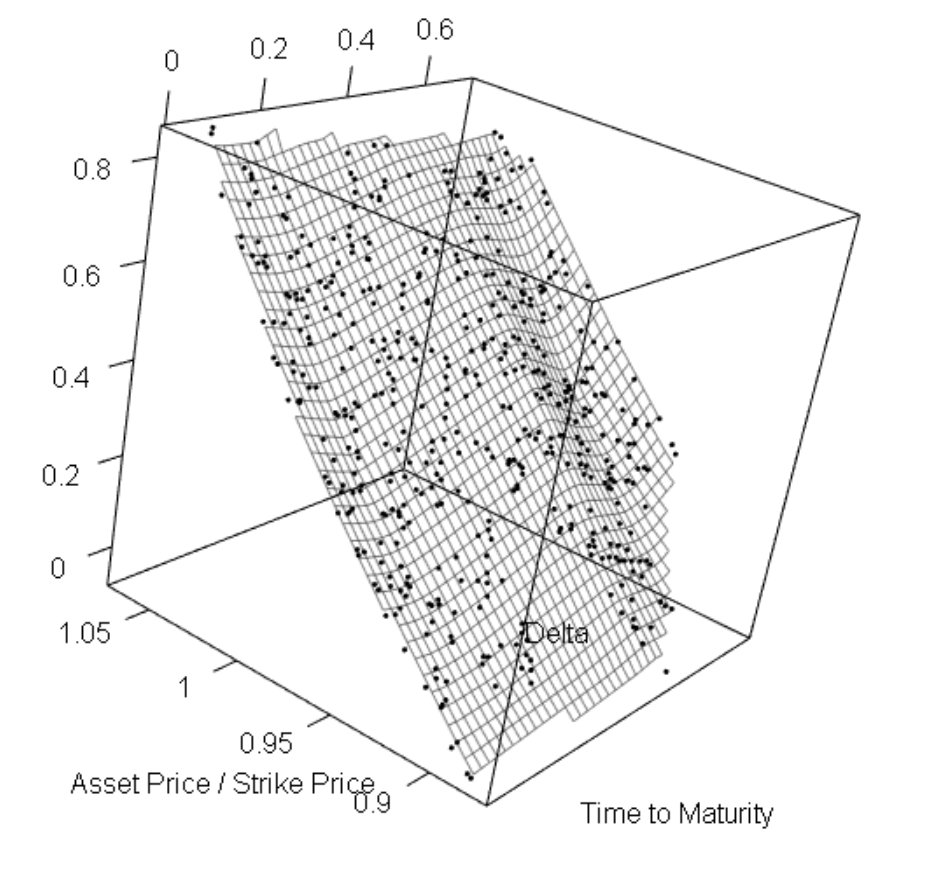
\includegraphics[width=0.7\linewidth]{Delta_pred.png}
	\centering
	\caption{Model estimate of BS delta (trained on delta)}
			\label{fig:Delta_pred}
\end{figure} 

\begin{figure}[p]
	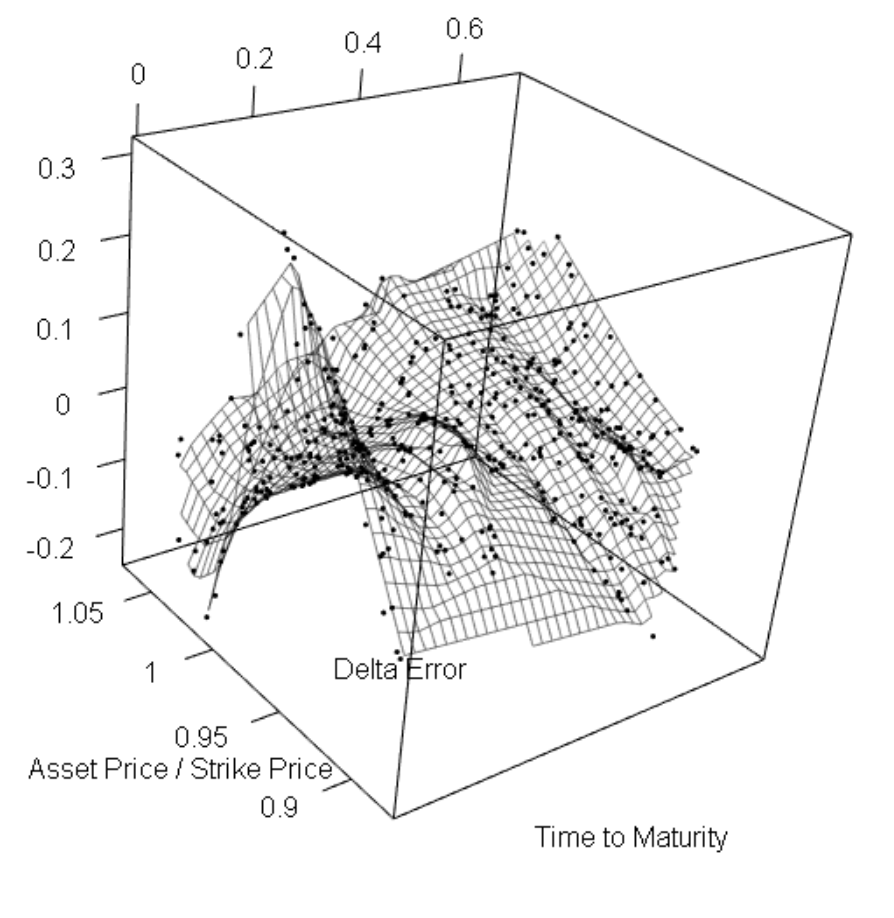
\includegraphics[width=0.7\linewidth]{Delta_err.png}
	\centering
	\caption{Model error of BS delta (trained on delta)}
			\label{fig:Delta_err}
\end{figure} 

\begin{figure}[p]
	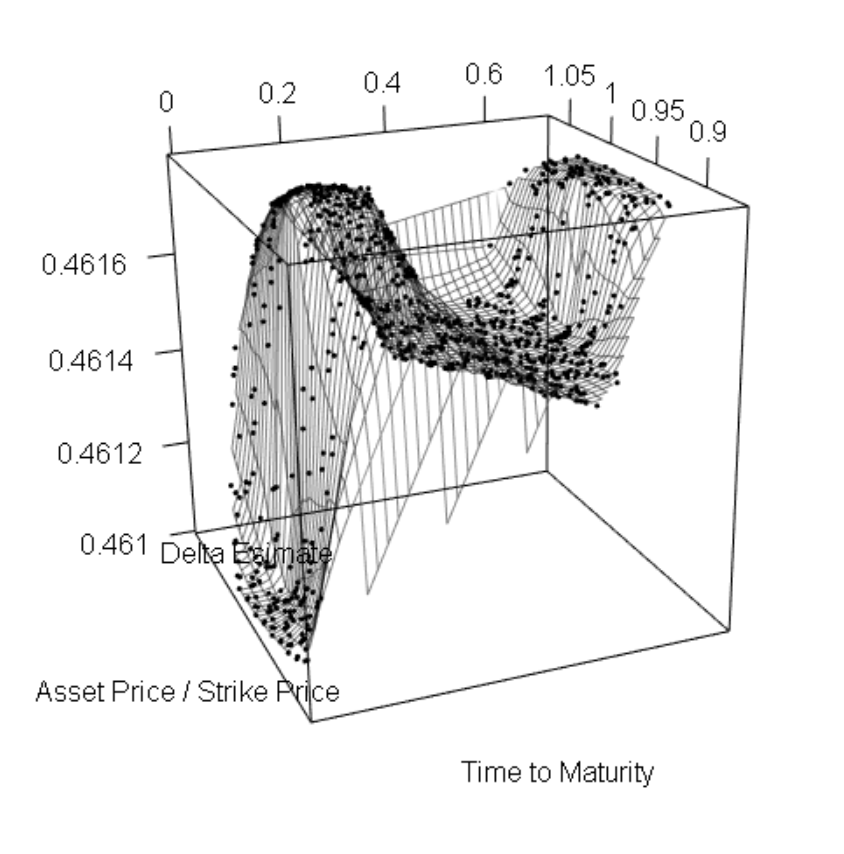
\includegraphics[width=0.7\linewidth]{Delta_derived.png}
	\centering
	\caption{Model estimate of BS delta (trained on BS call price)}
			\label{fig:Delta_derived}
\end{figure} 

\begin{figure}[p]
	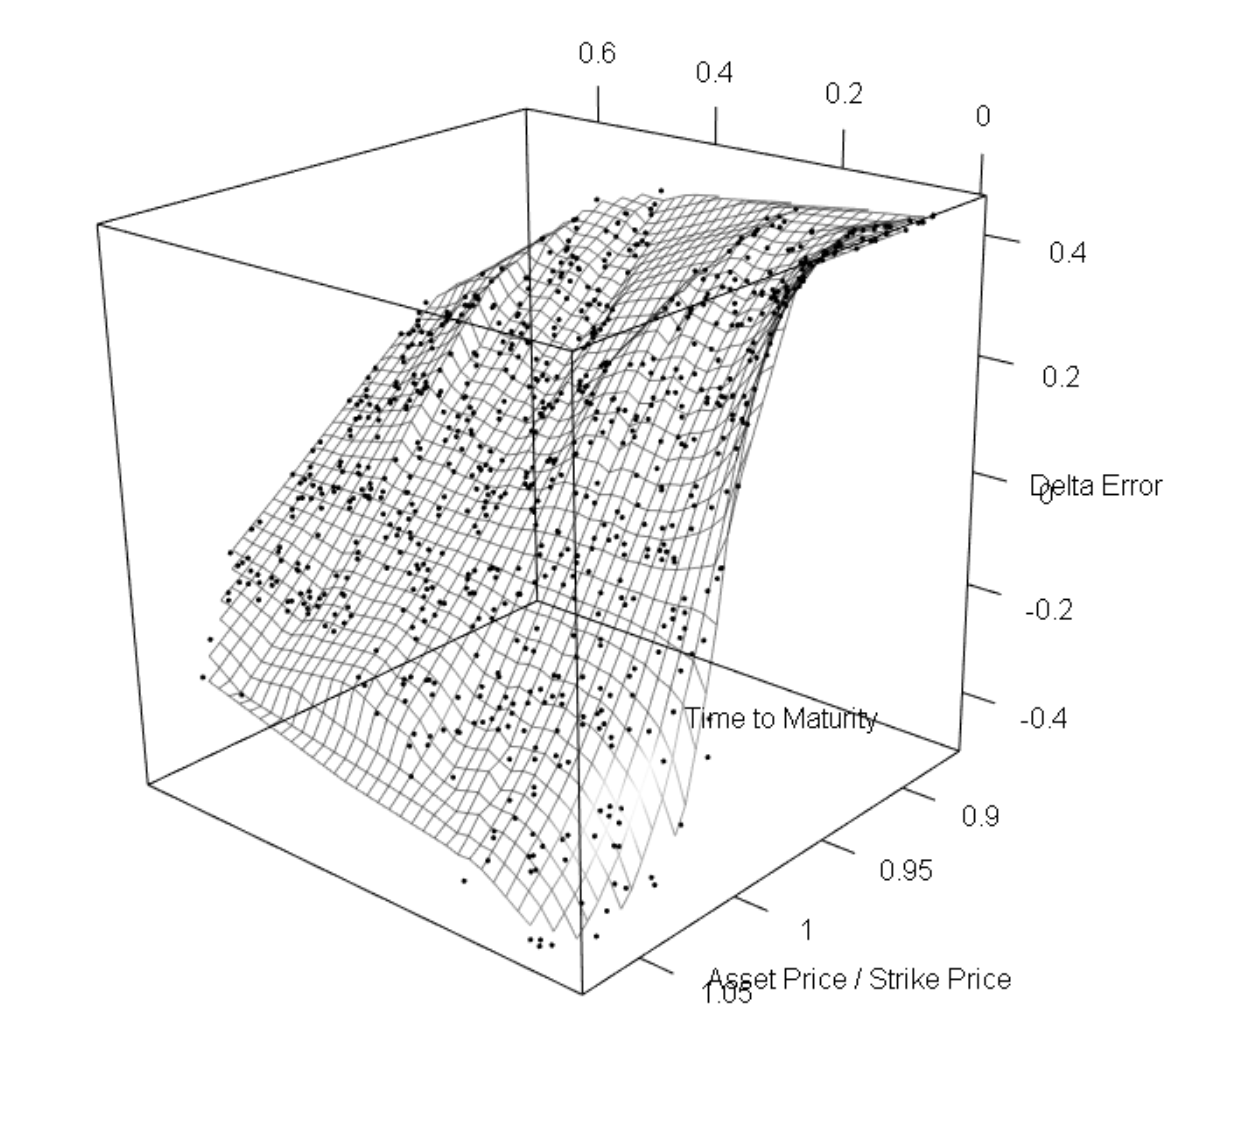
\includegraphics[width=0.7\linewidth]{Delta_err_derived.png}
	\centering
	\caption{Model error of BS delta (trained on BS call price)}
			\label{fig:Delta_derived_err}
\end{figure} 

 \clearpage 
\bibliographystyle{abbrv}
\bibliography{sigproc}  % sigproc.bib is the name of the 



\end{document}